\renewcommand\thesection{\Roman{section}}

\section{In the main idea, it is not clear the sampling proportion between the data from known and unknown classes. How does this proportion affect the subsequent training?}
\label{Question: class number}
\subsection*{\underline{\textbf{Response:}}}

As you mentioned, it is essential to indicate the affection of proportion between the data from known and unknown classes in the setting of open set domain adaptation.
However, in real scenarios, we can not manually set the sampling proportion due to the lack of target label information.
During the training phase, ThDAN is confined to randomly sample training data from the target domain.
So we conduct experiments to implicitly change the sampling proportion by varying the number of unknown data and the number of unknown classes.
All experiments are conducted on Office-31 datasets.
The following figures show the classification results.
\begin{figure*}[htb]
    \centering
    \subfloat[\footnotesize Accury \textit{w.r.t.} number of classes that are treated as the unknown]{
        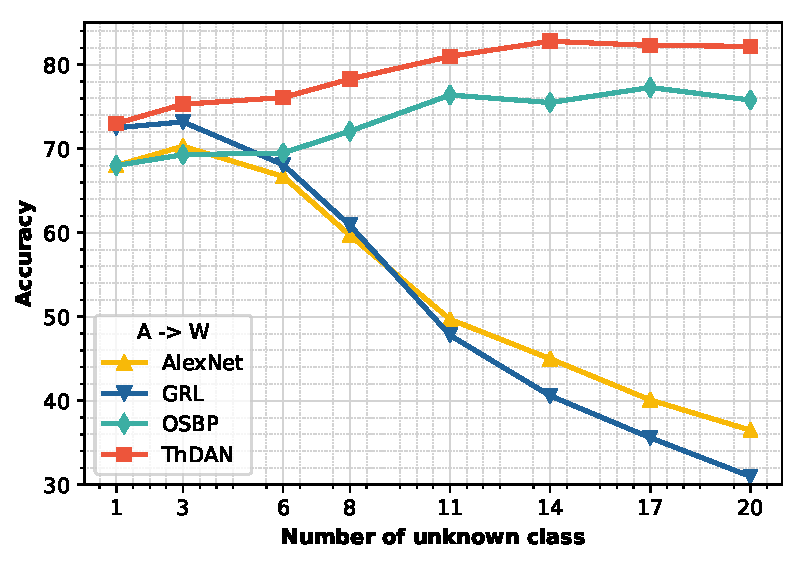
\includegraphics[width=0.33\textwidth]{contents/figures/pdf/analysis/class_change.pdf} 
        \label{figure: number of unknown class f}
    }
    \subfloat[\footnotesize Accury \textit{w.r.t.} ratio of used unknown samples]{
        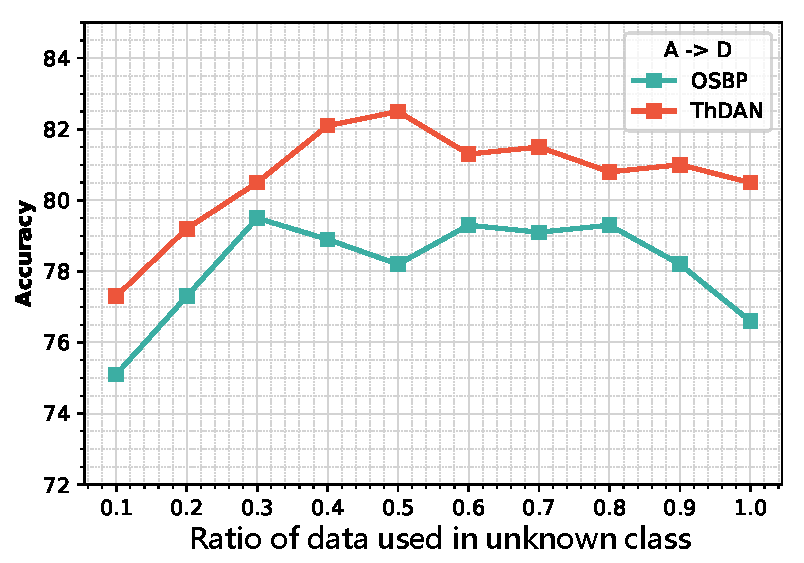
\includegraphics[width=0.34\textwidth]{contents/figures/pdf/analysis/nuknown_change.pdf} 
        \label{figure: ration of unknown f}
    } 
    \\
    \caption{
        (\textbf{a}): 
        The accuracy when we change the ratio of unknown samples in the adaptation task \textit{A$\to$D}. 
        (\textbf{b}): 
        The accuracy when we change the number of classes that are treated as the unknown in the adaptation task \textit{A$\to$W}. 
    }
    \label{figure: analysis change ratio}
\end{figure*}


We first fix the number of unknown classes to 10, and then change the sample number of each unknown class.
\textbf{Ratio 0.1} of sample number indicates that only one-tenth samples of each unknown class are used for training and testing, while the others are discarded from the dataset.
\figurename{\ref{figure: ration of unknown f}} shows the result.
When the ratio is low, the model can hardly identify samples from the unknown class due to the lack of training samples.
On the contrary, when the ratio is high, the negative effect of the unknown class will deteriorate the accuracy of categorizing known classes. 
Therefore the performance of the model is defective around the endpoint of the interval.

We further vary the number of unknown classes in \figurename{\ref{figure: number of unknown class f}}.
As the number of unknown classes increases, the performance of the methods proposed for close set domain adaptation will decrease significantly.
That is because they cannot alleviate the negative transfer brought by the unknown class.
The model proposed for open set domain adaptation would gain performance improvement by correctly rejecting samples of the unknown class.
This is because it is easier to reject samples as the ``unknown'' than categorize samples from the diverse known classes.
The accuracy tends to decay since too many unknown classes will deteriorate the process of knowledge transferring for the known classes.

The experiments show that the sampling proportion between the data from known and unknown classes could substantially affect model training for both unknown and known classes.
The low proportion of samples from unknown classes will affect the ability to identify samples from the unknown class.
On the other hand, the high proportion of that will affect the ability to classify samples from known classes.

\section{From their reported results in \textcolor{blue}{Fig.7}, the adjust threshold of $\gamma_0$ is not sensitive to the accuracy of training, it is a bit strange.  
Authors are encouraged to carefully check their claims by using more detailed reasons or more diverse data sets. }
\label{Question: threshold}
\subsection*{\underline{\textbf{Response:}}}

Thanks for your suggestions.
In our model, the threshold is calculated by averaging the transferability score of a batch of source samples and the predefined $\gamma$ as follows,
\begin{equation}
    \label{eq: transferability thresholded}
    \beta(X_s, \gamma) = \mathbb{E}_{x \in X_s} w(x) - \gamma.
\end{equation}

Then we dynamically increase $\gamma$ from $0$ to $\gamma_0$ so that more samples can be selected for domain adversarial training.
The changing function of $\gamma$ is as follows,
\begin{equation}
    \label{eq: dynamic tolerable range}
    \begin{split}
        \gamma &=
        \begin{cases}
            0 & ,\: n \in N_1 \\
            \gamma_0 \times  \sigma(n) & ,\: n\in N_2 \\
        \end{cases}.
    \end{split}
\end{equation}
Here $\sigma$ is a \textit{monotonically increasing function} with an upper bound of $1$.
$N_1$ and $N_2$ denote different training stage.

In experiments, we verify that the model is insensitivity to the value of $\gamma_0$ on \textbf{6 tasks of Office-31} and \textbf{12 tasks of Office-Home}.
We include \textcolor{blue}{Fig.7} of the original paper as follows, which shows the average prediction accuracy on these tasks when $\gamma_0$ changes,
\begin{figure}[htb]
    \centering
    \subfloat[Accury \textit{w.r.t.} the value of $\gamma_0$]{
        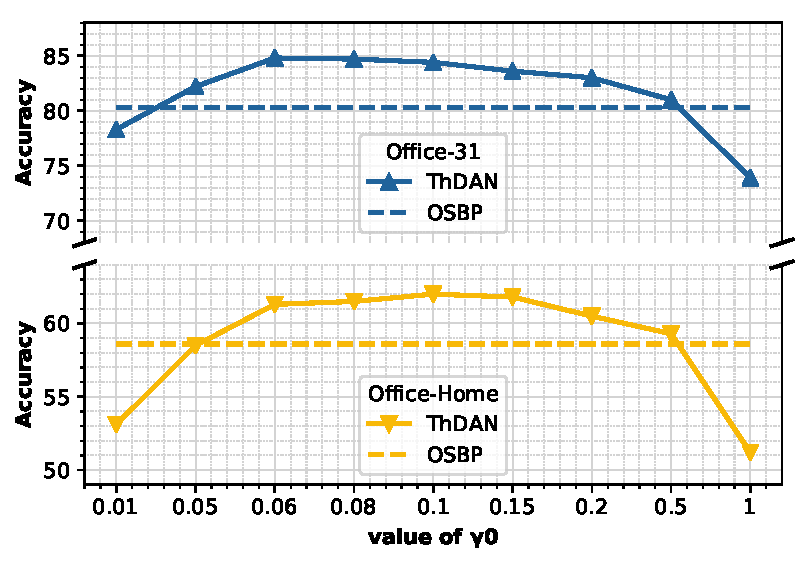
\includegraphics[width=0.33\textwidth]{contents/figures/pdf/analysis/sigma_change.pdf} 
        \label{figure: analysis in question 2}
    }
    \\
    \caption{
        The prediction accuracy of our method when we change the value of $\gamma_0$ on dataset Office-31 and Office-Home. 
    }
\end{figure}

Compared with the baseline model OSBP, our model can deliver plausible results on both Office-31 and Office-Home datasets when $\gamma_0$ in the range of $[0.06, 0.5]$.
That is because when we gradually increase the $\gamma$ during training, we also gradually decrease the learning rate.
As a result, the transferable samples selected in the early stage would ``dominate'' the model training, because they engage in training sooner, and the gradient produced by them can update the model with a larger learning rate.
As the $\gamma$ approaches $\gamma_0$, the learning rate is relatively low, and the previously selected samples would still be selected for training; therefore, the newcomers have little impact on model performance.
This directly reflects on the insensitivity of value of $\gamma_0$ to the accuracy of training.

The above explanation has been added in the revised manuscript.
Please refer to Section \textit{5.3.6} in the revised manuscript for details.

\renewcommand\thesection{\arabic{section}}
\setcounter{section}{0}

\section{The abstract needs to be redesigned.
    Open set domain adaptation (OSDA) should be a scenario.
    Authors claim to solve the OSDA problem. What is the problem?? This is unclear.
    It seems the author should firstly explain the OSDA setting and then present which issue they want to address. The first sentence of the abstract is a bit far away from their focus.
    More seriously, the introduction don not connect the abstract.
    For example, the beginning of the abstract explains the unsupervised domain adaptation, but the beginning of the introduction suddenly use deep learning to start this paper without unsupervised domain adaptation.
    Authors are encouraged to carefully reorganize their work, where the introduction must connect the abstract tightly.
    One sentence in the abstract should connect one logic in the introduction section.}
\subsection*{\underline{\textbf{Response:}}}


Thanks for your comments, the suggestions are of great help to improve our work.
In the revised manuscript, we redesigned the \textbf{abstract} and \textbf{introduction} for tighter logical connections.

The \textbf{abstract} has being redesigned as follows,
\begin{siderules}
    \textit{
        \footnotesize
        In recent years, many unsupervised domain adaptation (UDA) methods have been proposed to tackle the domain shift problem.
        Most existing UDA methods are derived for Close Set Domain Adaptation (\textit{CSDA}) in which source and target domains are assumed to share the same label space.
        However, target domain may contain unknown class different from the known ones in the source domain in practice, i.e., Open Set Domain Adaptation (\textit{OSDA}).
        Due to the presence of unknown class, aligning the whole distribution of the source and target domain for OSDA as in the previous methods will lead to negative transfer.
        Existing methods developed for OSDA attempt to assign smaller weights to target samples of unknown class.
        Despite promising performance achieved by existing methods, the samples of the unknown class are still used for distribution alignment, which make the model suffer from the risk of negative transfer.
        Instead of reweighting, this paper presents a novel method namely Thresholded Domain Adversarial Network (\textit{ThDAN}), which progressively selects transferable target samples for distribution alignment.
        Based on the fact that samples from the known classes must be more transferable than target samples of the unknown one, we derive a criterion to quantify the transferability by constructing classifiers to categorize known classes and to discriminate unknown class.
        In ThDAN, an adaptive threshold is calculated by averaging transferability scores of source domain samples to select target samples for training.
        The threshold is tweaked progressively during the training process so that more and more target samples from the known classes can be correctly selected for adversarial training.
        Extensive experiments show that the proposed method outperforms state-of-the-art domain adaptation and open set recognition approaches on benchmarks.
    }
\end{siderules}

According to the redesigned abstract, we have modified the \textbf{introduction} to make it connect to the abstract tightly.
The following Table \ref{table: logical} shows the logical connection between each paragraph of the introduction and each sentence of the abstract.
% Please add the following required packages to your document preamble:
% \usepackage{multirow}

% \newcommand\iw{0.05}
% \newcommand\cw{0.05}
% \renewcommand\tabularxcolumn[1]{m{#1}}
\newcommand\emmax[1]{\textcolor{red}{\textbf{#1}}}
\newcommand\methodyear[1]{\textcolor{blue}{#1}}
\newcommand\Tstrut{\rule{0pt}{2.6ex}}
\newcommand\Bstrut{\rule[-0.9ex]{0pt}{0pt}}

\newcommand{\centeritem}[1]{\noindent\parbox[c]{\hsize}{\footnotesize \vspace*{1mm} #1 \vspace*{1mm}}}

\begin{table*}[htb]
    \renewcommand{\arraystretch}{1.3}
    \caption{ The logical connection between paragraphs of the introduction and sentences of the abstract. }
    \label{table: logical}
    \centering
    \small
    % >{\itshape
    \begin{tabularx}{0.95\textwidth}{c| >{\itshape}X}
        \toprule[0.8pt]
        \textbf{\small Paragraph of Introduction} & \multicolumn{1}{c}{\textbf{\small Sentence of Abstract}}                                                                                                                                                                                                                              \\
        \bottomrule[0.8pt]
        \# 1             & \centeritem{In recent years, many unsupervised domain adaptation (UDA) methods have been proposed to tackle the domain shift problem.}                                                                                                          \\
        \hline
        \# 2             & \centeritem{Most existing UDA methods are derived for Close Set Domain Adaptation (\textit{CSDA}) in which source and target domains are assumed to share the same label space.
            However, target domain may contain unknown class different from the known ones in the source domain in practice, i.e., Open Set Domain Adaptation (\textit{OSDA}).}                                                                                            \\
        \hline
        \# 3             & \centeritem{Existing methods developed for OSDA attempt to assign smaller weights to target samples of unknown class.
            Despite promising performance achieved by existing methods, the samples of the unknown class are still used for training, which make the model suffer from the risk of negative transfer.}                                                                     \\
        \hline
        \# 4             & \centeritem{Instead of reweighting, this paper presents a novel method namely Thresholded Domain Adversarial Network (\textit{ThDAN}), which progressively selects transferable target samples for distribution alignment. ......} \\
        \bottomrule[0.8pt]
    \end{tabularx}
\end{table*}




\section{What is ``transferable''? How to evaluate it? Any definition to support this term?}
\label{question: transferable}
\subsection*{\underline{\textbf{Response:}}}

Unfortunately, there is no formal definition or mathematical formula to define ``transferable'' in the context of domain adaptation.
Generally, the word ``transferable' is used to describe features.
Here we quote from \cite{DeepAdaptationNetworks}:
\begin{quote}
    \textit{the transferable features are the features that generalize well to novel tasks for domain adaption}
\end{quote}
While the later work \cite{TransferableAttentionDA} also uses ``transferable'' to describe samples that contribute to the transfer task of domain adaptation.

In the scenario of open set domain adaptation, we consider the target samples from the known classes are transferable samples since they can boost the classification performance of the model.
On the contrary, the target samples from the unknown class are considered as untransferable samples, that is because aligning distribution with them will incur negative transfer.

In this work, we evaluate transferability based on two observations:

\textbf{Target samples from the known classes are able to confuse $G_d$.}
Here $G_d$ is the domain discriminator that gives the probability of being target samples.
For a target sample, if $G_d(z)$ approaches to $1$, then the sample has a high probability of coming from the unknown class.
That is because the unknown class is only included in the target domain and can be almost perfectly discriminated from the source samples.
On the other hand, if $G_d(z)$ approaches to $0$, then the sample is more likely from the known classes that shared by domains.
Therefore the transferable target samples are able to confuse $G_d$ to label them as the source samples.
Then we can define the transferability $w_d(x)$ as inversely related to $G_d(z)$,
\begin{align}
    w_d(x) &= 1-G_d(z). \label{eq: domain transferability}
\end{align}

\textbf{Target samples from the known classes can be categorized by $G_{c, known}$.}
Here $G_{c, known}$ is the classifier that gives the probability distribution among known classes.
Due to the overlapping in the marginal distributions across domains, target samples from the known classes could be categorized correctly by the classifier $G_{c, known}$ that trained on the source samples. 
This leads to low entropy (high transferability) for the samples from the known classes.
For the samples from the unknown class, because they cannot be classified into one of the $K$ known classes, the uncertainty of the prediction measured by the entropy is large.
Therefore the transferability $w_c(x)$ can be defined as inversely related to the \textit{normalized} classification entropy $H$,
\begin{align}
    w_c(x) &=1-H(G_{c,\; known}(z)). \label{eq: class transferability}
\end{align}

Since the domain discriminate $G_d$ in Eq.(\ref{eq: domain transferability}) and the classifier $G_{c, known}$ in Eq.(\ref{eq: class transferability}) work independently, we can unify the transferability criterion as,
\begin{equation}
    \label{eq: transferability}
    w(x)=1-G_d(z)\cdot H(G_{c,\; known}(z)).
\end{equation}
The experiments in Section 4 show that the transferability criterion of Eq.(\ref{eq: transferability}) works well for our model to select target samples from the known classes.


\section{In \textcolor{blue}{Fig.1}, it is unclear why (d) must outperform the other methods.}
\subsection*{\underline{\textbf{Response:}}}

Thanks for your comments.
\textcolor{blue}{Fig.1} in the original manuscript is as follows,

\begin{figure}[H]
    \centering
    \subfloat{
        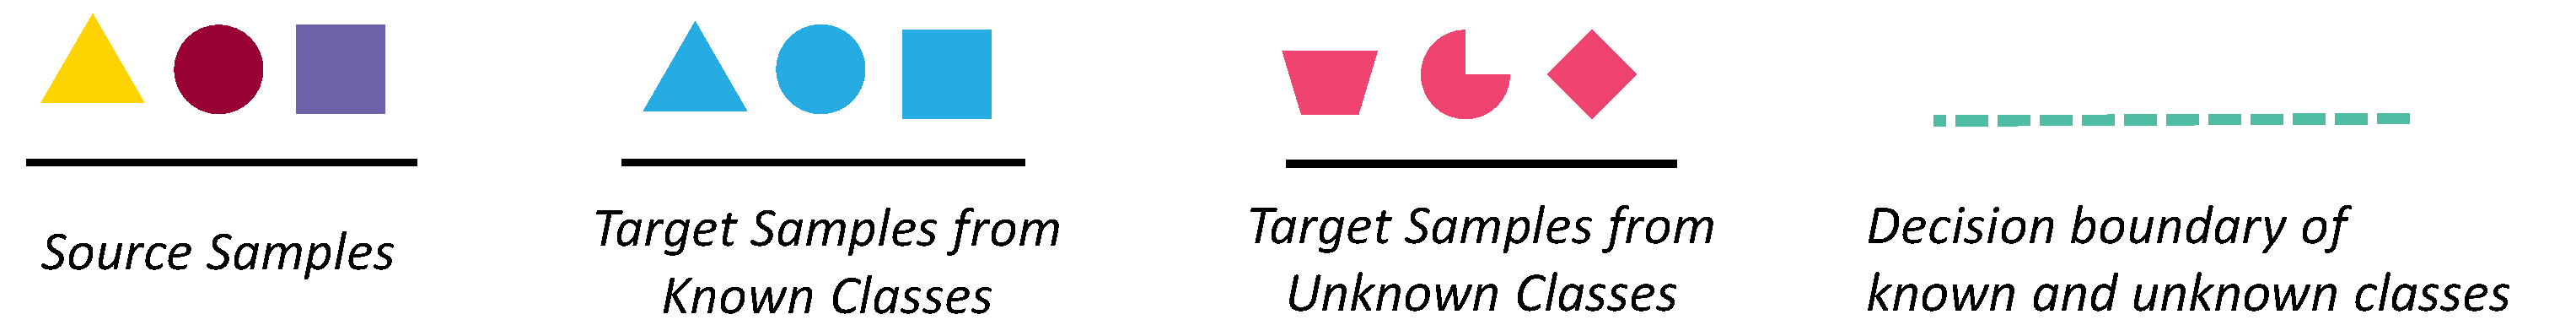
\includegraphics[width=0.55\textwidth]{contents/figures/pdf/overview/note.pdf} 
    }
    \\
    \addtocounter{subfigure}{-1}
    \subfloat[]{
        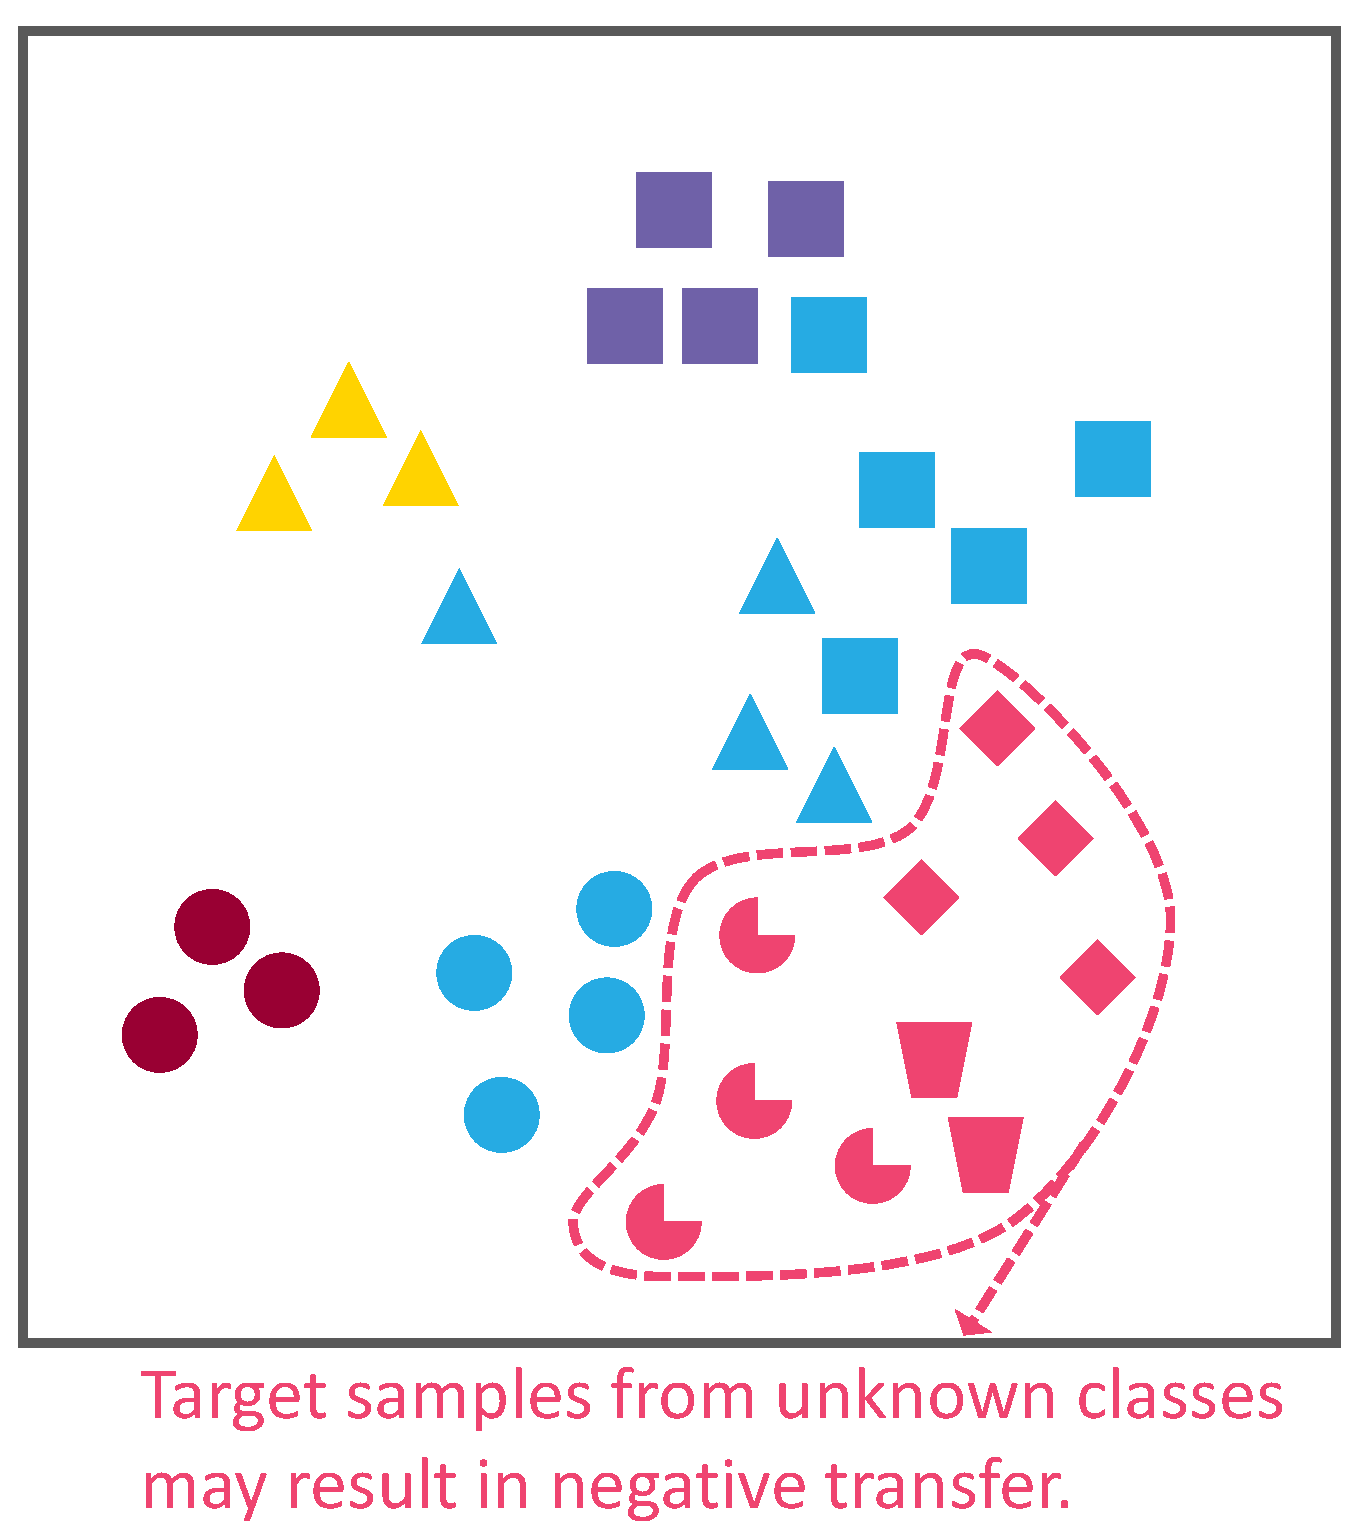
\includegraphics[width=0.22\textwidth]{contents/figures/pdf/overview/1.pdf} 
        \label{figure: reweighting based}
    } 
    \subfloat[]{
        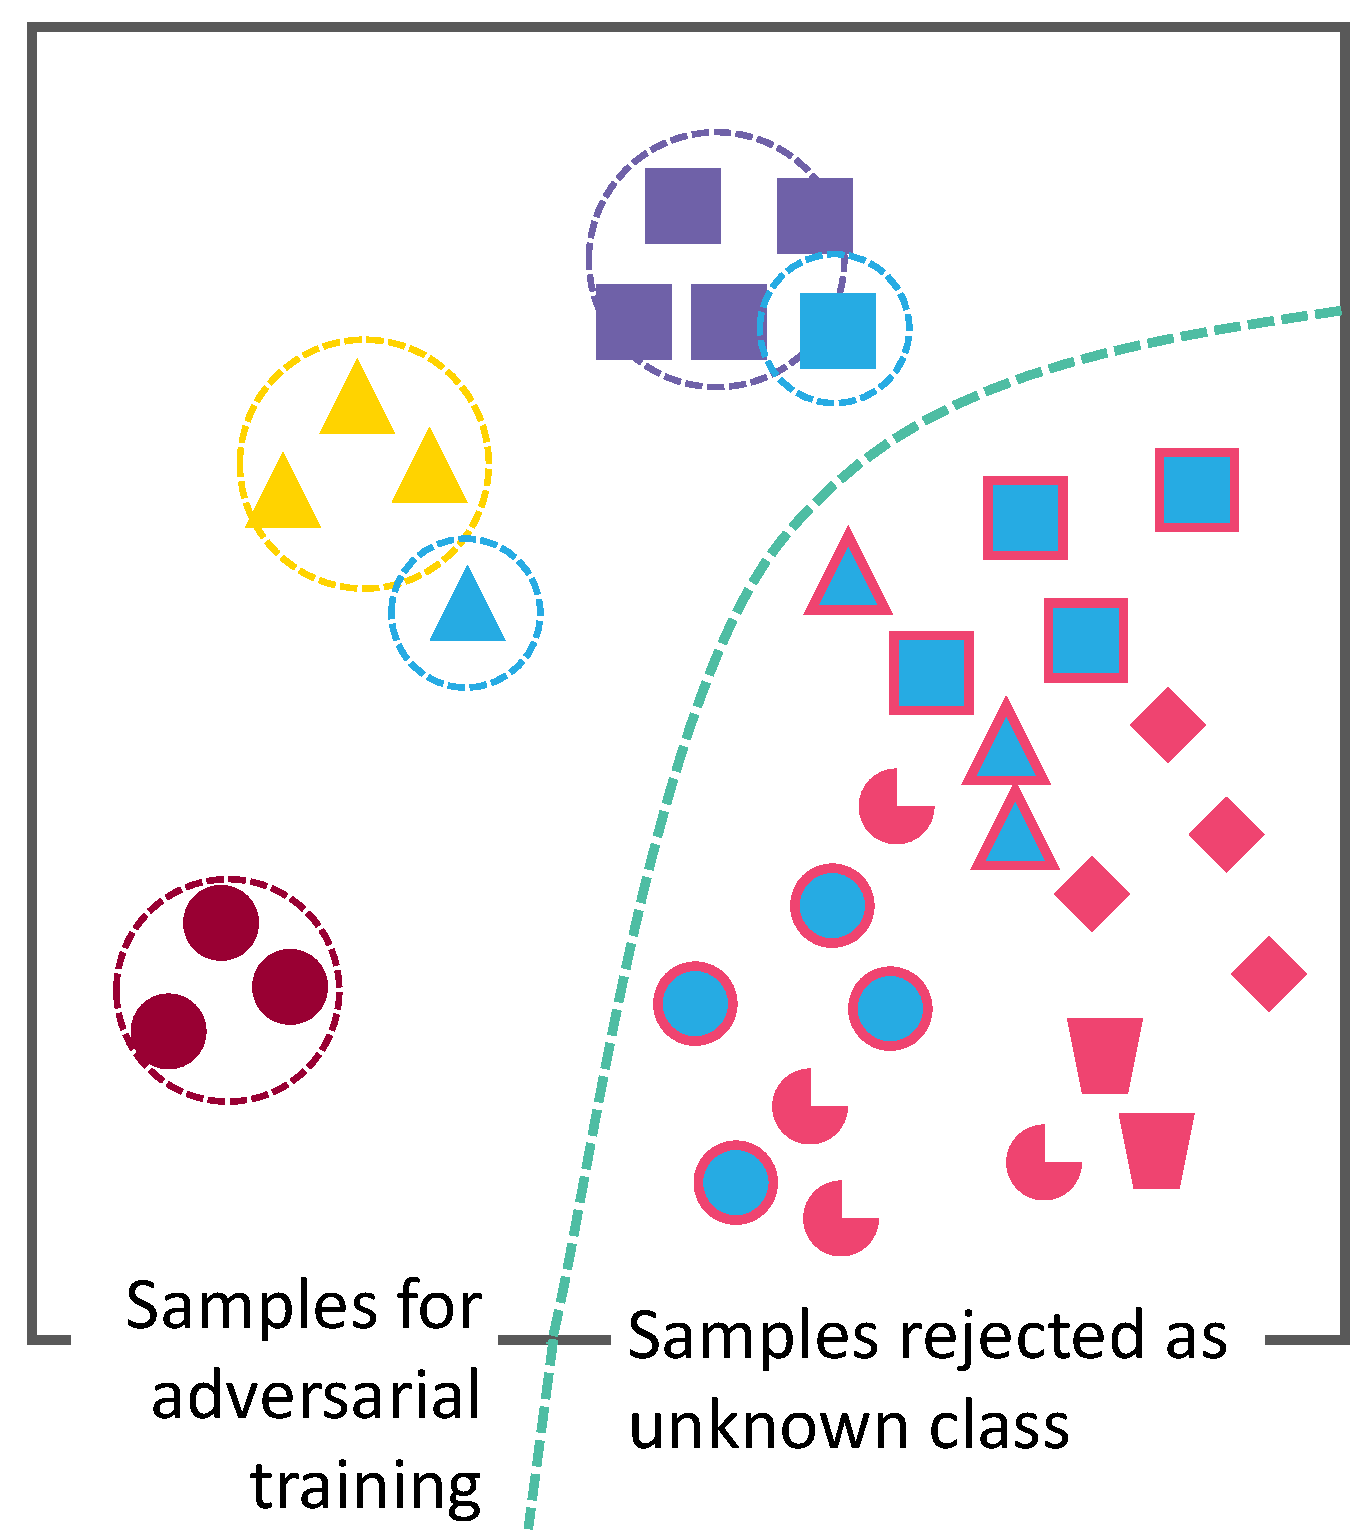
\includegraphics[width=0.22\textwidth]{contents/figures/pdf/overview/2.pdf} 
        \label{figure: ThDAN 1}
    } 
    \subfloat[]{
        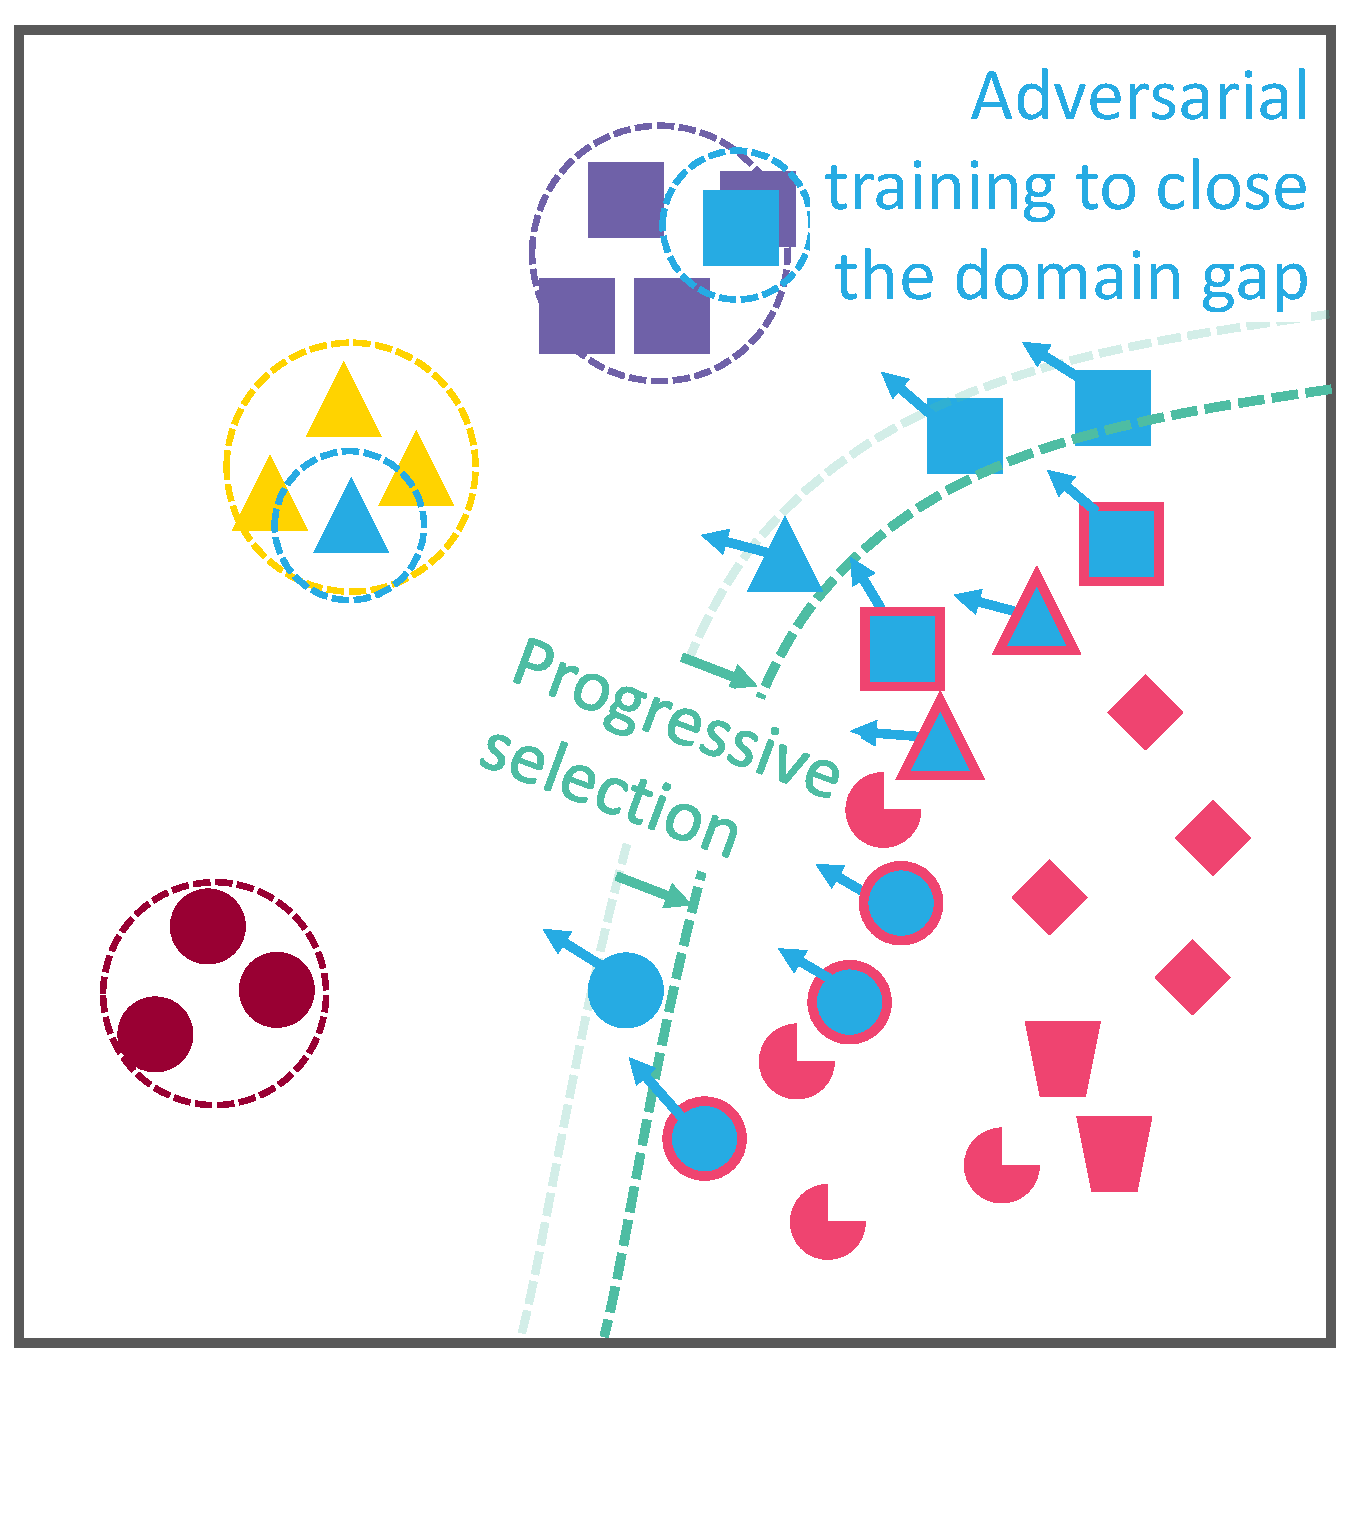
\includegraphics[width=0.22\textwidth]{contents/figures/pdf/overview/3.pdf} 
        \label{figure: ThDAN 2}
    } 
    % \hfil
    \subfloat[]{
        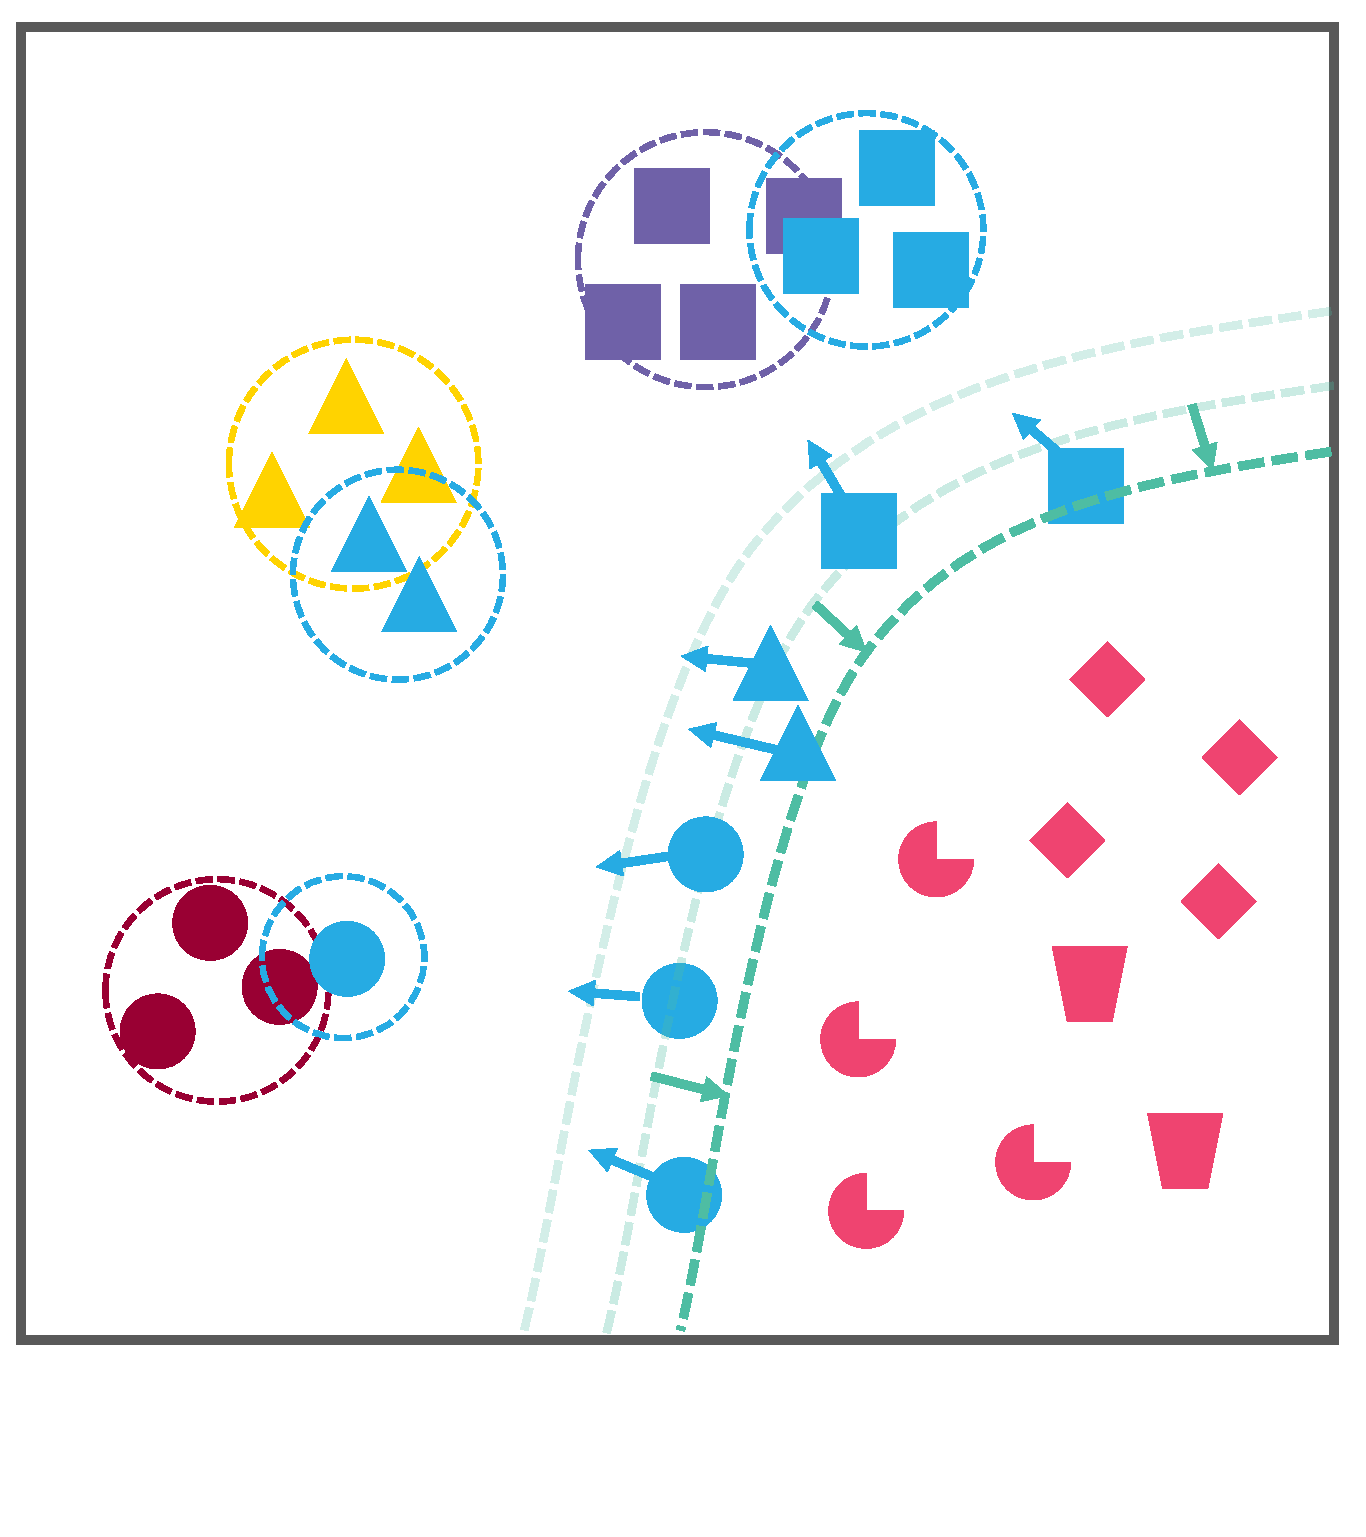
\includegraphics[width=0.22\textwidth]{contents/figures/pdf/overview/4.pdf} 
        \label{figure: ThDAN 3}
    }
    \caption{
        Figure1 of the original manuscript.
    } 
    \label{figure: overview} 
\end{figure}



As a matter of fact, \figurename{\ref{figure: overview}} illustrates the general idea of the proposed method.
To make a clearer presentation for \figurename{\ref{figure: overview}}, we modify the caption in the revised manuscript as follows,
\begin{siderules}
    \textit{
        \footnotesize
        The general idea of the proposed Thresholded Domain Adversarial Network (\textit{\textbf{ThDAN}}).
        (\textbf{a}): Training samples for open set domain adaptation. 
        (\textbf{b}): ThDAN builds a decision boundary based on the transferability threshold to separate known and unknown classes.
        (\textbf{c}): ThDAN aligns the distributions of the source and the samples selected as known classes. Then ThDAN tweaks the transferability threshold to collect more samples of known classes to enhance distribution alignment.
        (\textbf{d}): ThDAN progressively selects more samples of the known classes for training. All the unselected samples are rejected as ``unknown''.
    }
\end{siderules}


\section{What is ``domain-invariant features'' ?}
\subsection*{\underline{\textbf{Response:}}}

In domain-invariant feature space, the source and target domains have the same (or similar) marginal distributions, and the posterior distributions of the labels are the same across domains too \cite{DeepDomainConfusion}.
Hence, a classifier trained on the labeled source domain would likely perform well on the target domain.

Specifically, the domain-invariant features can be obtained by performing \textit{domain adversarial training} \cite{DomainAdversrialNetwork,ADDA,OpensetDA-bp}.
The domain adversarial training is a minmax game: a domain discriminator is trained to separate the feature representation of the source domain from the one of the target domain, at the same time, feature generators are trained to deceive the domain discriminator.
In this work, we adopt the training scheme proposed in \cite{OpensetDA-bp} to enable the domain discriminator to identify samples of unknown class for open set domain adaptation. 
Formally, the training procedure can be written as,
\begin{equation}
    \label{eq: training DANN}
    \begin{split}
        \min_{G_f^t} \max_{G_d} \mathscr{L}(G_d,G^{s}_{f},G_f^t) &=\mathbb{E}_{x\sim p_t(x)} \left[ \log \left(G_d\left(G_f^t\left(x\right)\right)\right) \right]\\
        &+\mathbb{E}_{x\sim p_s(x)}\left[ \log \left(1-G_d\left(G_f^s\left(x\right)\right)\right) \right].
    \end{split}
\end{equation}
$G_f^s$ and $G_f^t$ are the feature extractors for source and target samples, which share weights as in \cite{OpensetDA-bp}.
$G_d$ aims to label source samples as $0$ and target samples as $1$.
The optimization of Eq.(\ref{eq: training DANN}) makes $G_f$ to generate features that can not be discriminated by $G_d$ (\textit{i.e.,} domain-invariant features).
Therefore the classifier $G_c$ that trained on the source domain can perform well for target samples by leveraging features extracted by $G_f$.

\section{In the related work, CSDA does not have references.}
\subsection*{\underline{\textbf{Response:}}}
Thanks for your suggestion.
CSDA is referred to Close Set Domain Adaptation and we have add references \cite{ben2010theory,Elsevier-DeepVisualDA,TransferLearningSurvey} for the methods for CSDA in the revised manuscript.

\section{In section 2.1, "Another way to solve domain adaptation" is not suitable. 
Domain adaptation is a setting in detailed ML tasks or a probability distribution issue. 
Authors can obtain more information from S Ben-David's paper.}
\subsection*{\underline{\textbf{Response:}}}
Thanks for your comment.
We agree that the phrase ``Another way to solve domain adaptation'' is not precise. 
This phrase is revised as ``Another approach for domain adaptation''. 
Similar unprecise wordings have been modified in the revised manuscript.
Also, we have carefully read Ben-David's paper \cite{ben2010theory} to get a better understanding of domain adaptation and has cited this paper in the revised manuscript.


\section{Section 2.2 missed some new work from open-set domain adaptation.}
\subsection*{\underline{\textbf{Response:}}}
Thanks for your suggestions.
We add some new work \cite{PDA-fac,PDA-sep} of open set domain adaptation in Section 2.2, they are respectively from ICML2019 and CVPR2019.

Furthermore, we implement \textit{Factorized Representations For Open Set Domain Adaptation \textbf{(FRFOSDA)}} model proposed in \cite{PDA-fac} in experiments on \textbf{Office-Hone} and \textbf{Office31} for comparisons.
Please refer to Section 4 for more details.

\section{In Section 3, authors missed the definition on $C_t$. Is it the label space of target domain?}
\subsection*{\underline{\textbf{Response:}}}
Yes, $C_t$ is the label space of target domain.
In the revised manuscript, the definition on $C_t$ has been added in section \textit{3.1 open set domain adaptation} as follows,
\begin{siderules}
$C_s$ and $C_t$ respectively denote the label space of the source and target domain.
In the setting of open set domain adaptation, the label space of target domain contains the label space of source domain, \textit{i.e.}, $C_s \subset C_t$. 
We refer to classes from from $C_s$ as the known classes and classes from $C_t\backslash C_s$ as the unknown class.
\end{siderules}


\section{In Section 3.1, what is ``untransferable ones''?}
\subsection*{\underline{\textbf{Response:}}}

This question is related to Question \ref{question: transferable}.
In the setting of open set domain adaptation, the untransferable ones refer to the samples of unknown class in the target domain.
The proposed method selects untransferable samples by evaluating transferability as follows,
\begin{equation}
    \label{eq: split target examples untrnasferable}
    \begin{split}
        X_t^u=\{x|w(x) < \beta, x \in X_t \}.
    \end{split}
\end{equation}
The $w$ is transferability calculator in Eq.(\ref{eq: transferability}), and $\beta$ is transferability threshold calculated by averaging and tweaking transferability scores of source samples.
The selection procedure indicated in Eq.(\ref{eq: split target examples untrnasferable}) shows that target samples  $X_t$ whose transferability smaller than the threshold will be selected as untransferable target samples $X_t^u$. 

\section{In \textcolor{blue}{Eq.(2)}, more strong reasons need to be presented to explain the $G_f$ and $G_d$. Why the use such settings to define them? Only based other's work?}
\subsection*{\underline{\textbf{Response:}}}

Thanks for your comments.
The reason why we use the setting ``{$G_f$ and $G_d$ can be considered as the generative network and discriminate network of GAN respectively'' to define $G_f$ and $G_d$ in \textcolor{blue}{Eq.(2)} is that the \textit{domain adversarial training} between $G_f$ and $G_d$ is similar to the original training procedure of \textit{Generative Adversarial Nets (GAN)} \cite{goodfellow2014generative}.
In GAN, the discriminate network $D$ and the generative network $G$ are trained with the following objective, 
\begin{equation}
    \label{eq: GAN}
    \begin{split}
        \min_G \max_D V(D,G) &= \mathbb{E}_{x\sim p_{data}(x)}[\log D(x)] \\ &+ \mathbb{E}_{z\sim p_z(z)}[\log (1-D(G(z)))]. 
    \end{split}
\end{equation}
In the training of GAN of Eq.(\ref{eq: GAN}), $D$ is trained to separate the feature representation of the true images and fake images, and $G$ is trained to generate fake images that can confuse $D$.
While in the domain adversarial training of Eq.(\ref{eq: training DANN}), $G_d$ is trained to separate the feature representation of the source domain from the target domain, and $G_f$ is trained to generated target features that are able to confuse $G_d$.
The training procedure for $D$ and $G$ is very similar to the domain adversarial training for $G_d$ and $G_f$. 
Therefore we can define $G_f$ and $G_d$ by the setting of GAN.

We think this setting is not convincing enough to explain why \textcolor{blue}{Eq.(2)} is the optimal $G_d$, and have removed it in the revised manuscript.
We have added more formal proof for Eq.(\ref{eq: revised optimal}) in the revised manuscript, please refer to the reply of the next question for details.

\section{In the following, why does $G_d$ converge to the optimal?}
\subsection*{\underline{\textbf{Response:}}}

\textcolor{blue}{Eq.(2)} is as follows,
\begin{equation}
    \label{eq: revised optimal}
    \begin{split}
        G_d^*(z) &= \frac{p_t(z)}{p_s(z)+p_t(z)}. \\
    \end{split}
\end{equation}

Here $z$ is the deep feature representation of a sample, \textit{i.e.,} $z=G_f(x)$.
We give the proof that Eq.(\ref{eq: revised optimal}) is the optimal $G_d$ for Eq.(\ref{eq: training DANN}) as follows,
\begin{proof}
    For any $G_f^s$ and $G_f^t$, we train $G_d$ to maximize Eq.(\ref{eq: training DANN}):
    \begin{equation}
        \label{eq: proof optimal discriminator}
        \begin{split}
            \max_{G_d} \mathscr{L}(G_d,G^{s}_{f},G_f^t)  = &\int_x p_t(x)\log \left(G_d\left(G_f^t\left(x\right)\right)\right)
              + p_s(x) \log\left(1-G_d\left(G_f^s\left(x\right)\right)\right) \, dx.
            \\ = &\int_z p_t(z)\log \left(G_d\left(z\right)\right)
              + p_s(z) \log\left(1-G_d\left(z\right)\right) \, dz.
        \end{split}
    \end{equation}
    We take the partial differential of the objective Eq.(\ref{eq: proof optimal discriminator}) with respect to $G_d$, and apply the Leibnizs rule to exchange the order of differentiation and integration to achieve optimal $G_d$ in $[0, 1]$ at Eq.(\ref{eq: revised optimal}).
\end{proof}

The proof has been added in Section 3.2 of the revised manuscript.

\section{In \textcolor{blue}{Eq.(2)}, how to define $p_s$ and $p_t$?}
\subsection*{\underline{\textbf{Response:}}}

\textcolor{blue}{Eq.(2)} is as follows,
\begin{equation}
    \label{eq: revised optimal 1}
    \begin{split}
        G_d^*(z) &= \frac{p_t(z)}{p_s(z)+p_t(z)}. \\
    \end{split}
\end{equation}
Here $z$ is the deep feature representation of a sample, \textit{i.e.,} $z=G_f(x)$.
As stated in \textit{Section 3.1 open set domain adaptation} of the revised manuscript, $p_s (z)$ and $p_t (z)$ are probability distributions of feature representations in source and target domains respectively, as defined in \cite{PartialDA-iw}.


\section{In \textcolor{blue}{Eq.(9)}, what is  $X_t^k$?}
\subsection*{\underline{\textbf{Response:}}}

Thanks for your comments.
The \textcolor{blue}{Eq.(9)} in the original manuscript is as follows,
\begin{equation}
    \label{eq: split target examples}
    \begin{split}
        X_t^k=\{x|w(x) \geq \beta, x \in X_t \}, \\
        X_t^u=\{x|w(x) < \beta, x \in X_t \}.
    \end{split}
\end{equation}
Here $X_t^k$ denotes the transferable target samples that are selected as the samples from the known classes.
And $X_t^u$ denotes the untransferable target samples that are regarded as the samples from the unknown class.
Specifically, in Eq.(\ref{eq: split target examples}), $\beta$ is a transferability threshold, $w$ is the transferability calculator.
For a batch of target training data $X_t$, we use the threshold $\beta$ to split it into two parts, $X_t^k$ and $X_t^u$.
For target samples in $X_t^k$, we train the model to align distribution with the source samples.
For target samples in $X_t^k$, we train the $G_d$ to identify them as ``unknown'' samples.

We added Section 4.1 in the revised manuscript to clarify the proposed methods and equations, in which $X_t^k$ and $X_t^u$ are explained.

\section{A same controversial issue appears again: Sample selection is the key step for this model to address open set domain adaptation.}
\subsection*{\underline{\textbf{Response:}}}

Thanks for pointing out the mistakes.
This sentence has been modified as ``The sample selection algorithm will substantially affect the performance of ThDAN for open set domain adaptation'' 

Similar mistakes have bee corrected in the revised manuscript.


\section{In the experiments, why do you use different setting to begin the experiments in Section 4.2.1? Authors are encouraged to explain the inherent reasons.}
\subsection*{\underline{\textbf{Response:}}}

Thanks for your suggestions.
We want to use different settings to perform ablation studies to evaluate the efficacy of the threshold tweaking techniques proposed in Section 4.5.
The ablation studies on Office-31, OfficeHome and VisDA datasets involve 3 kinds of ThDAN variants.
(\textbf{1}) \textit{\textbf{ThDAN-m-dy}} is the original setting which calculates transferability threshold based on mini-batch samples and a fixed $\gamma$.
(\textbf{2}) \textit{\textbf{ThDAN-dy}} is the variant applies exponential moving average to update transferability threshold.
(\textbf{3}) \textit{\textbf{ThDAN}} further takes advantage of dynamic $\gamma$ to tweak transferability threshold.

In order to better understand how the proposed method performs under ablation settings, we add Section \textit{5.3.1 Ablation Study} in the revised manuscript.
Please refer to the revised manuscript for details.


\section{A same issue appear again in the settings of Section 4.2.2.}
\subsection*{\underline{\textbf{Response:}}}

Thanks for your comments.
This question is related to the previous question.
In the revised manuscript, the ablation study in the original \textcolor{blue}{Section 4.2.2} has been reorganized in \textit{Section 5.3.1 Ablation Study}.


\section{The results analysis in Section 4.2.3 is unclear. More detailed reasons need to be present to support your conclusion.}
\subsection*{\underline{\textbf{Response:}}}

The results of \textcolor{blue}{Section 4.2.3} are as follows,
% Please add the following required packages to your document preamble:
% \usepackage{multirow}

% \newcommand\iw{0.05}
% \newcommand\cw{0.05}
% \renewcommand\tabularxcolumn[1]{m{#1}}
\newcommand\emmax[1]{\textcolor{red}{\textbf{#1}}}
\newcommand\methodyear[1]{\textcolor{blue}{#1}}
\newcommand\Tstrut{\rule{0pt}{2.6ex}}
\newcommand\Bstrut{\rule[-0.9ex]{0pt}{0pt}}

\begin{table*}[htb]
    \renewcommand{\arraystretch}{1.3}
    \caption{Accuracy (\%) of each method with 6 shared class on VisDA. }
    \label{table: exp on visDA}
    \centering
    \small
    \begin{tabularx}{0.95\textwidth}{r Y Y Y Y Y Y Y >{\itshape}Y >{\itshape}Y }
        \toprule[0.8pt]
        \multicolumn{1}{c}{\multirow{2}{*}{Method}} & \multicolumn{9}{c}{  class-wise accuracy on VisDA}                                                                       \\ \cmidrule[0.1pt]{2-10}
        \multicolumn{1}{c}{}                        & Bcycle                                             & Bus  & Car  & Mcycle & Train & Truck & Unkown & Avg.All & Avg.Known \\
        \hline
        OSVM  \methodyear{[ECCV, 2014]}                                      & 4.8                                                & 45.0 & 44.2 & 43.5   & 59.0  & 10.5  & 57.4   & 37.8    & 34.5      \\
        MMD  \methodyear{[NIPS, 2007]}                                  & 0.2                                                & 30.9 & 49.1 & 54.8   & 56.1  & 8.1   & 61.3   & 37.2    & 33.2      \\
        GRL  \methodyear{[JMLR, 2016]}                                   & 9.1                                                & 50.5 & 53.9 & 79.8   & 69.0  & 8.1   & 42.5   & 44.7    & 45.1      \\
        OSBP  \methodyear{[ECCV, 2018]}                                       & 48.0                                               & 67.4 & 39.2 & 80.2   & 69.4  & \emmax{24.9}  & 80.3   & 58.5    & 54.8      \\
        \hline
        ThDAN-dy                                    & 52.6                                               & 69.5 & 58.8 & 83.1   & 72.3  & 12.3  & 84.5   & 61.8    & 58.1      \\
        ThDAN                                 & \emmax{55.2}                                               & \emmax{70.8} & \emmax{61.4} & \emmax{85.6}   & \emmax{74.8}  & 10.0  & \emmax{88.8}   & \emmax{63.8}    & \emmax{59.6}      \\
        \bottomrule[0.8pt]
    \end{tabularx}
\end{table*}



In the experiments of VisDA, the training split is used as the source domain and validation one as the target domain.
We choose 6 categories, i.e., bicycle, bus, car, motorcycle, train and truck as the known classes, and the other 6 categories as the unknown class.
As Table. \ref{table: exp on visDA} shows the classification results, where \textit{Avg.All} and \textit{Avg.Known} indicate the accuracy averaged over all classes and known classes.
For the classification of known classes, ThDAN can exceed other methods in almost every class and in the average, which means our method can effetely transfer knowledge for the classification task.
This is because ThDAN can avoid the negative transfer by only selecting transferable target samples for domain adversarial training.
Also, our model improves the classification accuracy for the unknown class by a big margin.
This further verifies the efficiency of the sample selection algorithm, since ThDAN will reject the unselected samples as the unknown class.

The analysis mentioned above has been added to the corresponding section in the revised manuscript.

\section{Please carefully check the claim in \textcolor{blue}{Fig.7}.}
\subsection*{\underline{\textbf{Response:}}}

Thanks for your reminding.
The \textcolor{blue}{Fig.7} in the original manuscript is as follows,
\begin{figure}[H]
    \centering
    \subfloat[\footnotesize Accury \textit{w.r.t.} ratio of used unknown samples]{
        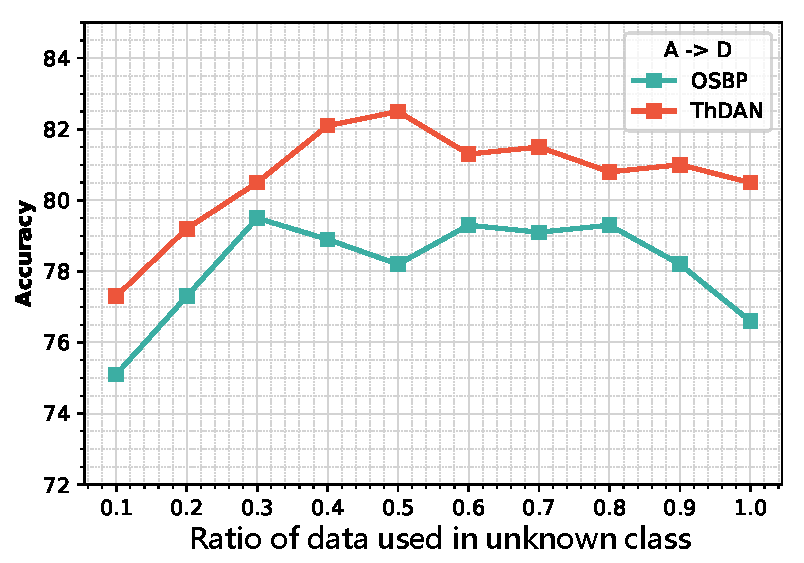
\includegraphics[width=0.34\textwidth]{contents/figures/pdf/analysis/nuknown_change.pdf} 
        \label{figure: ration of unknown}
    } 
    \subfloat[\footnotesize Accury \textit{w.r.t.} number of classes that are treated as the unknown]{
        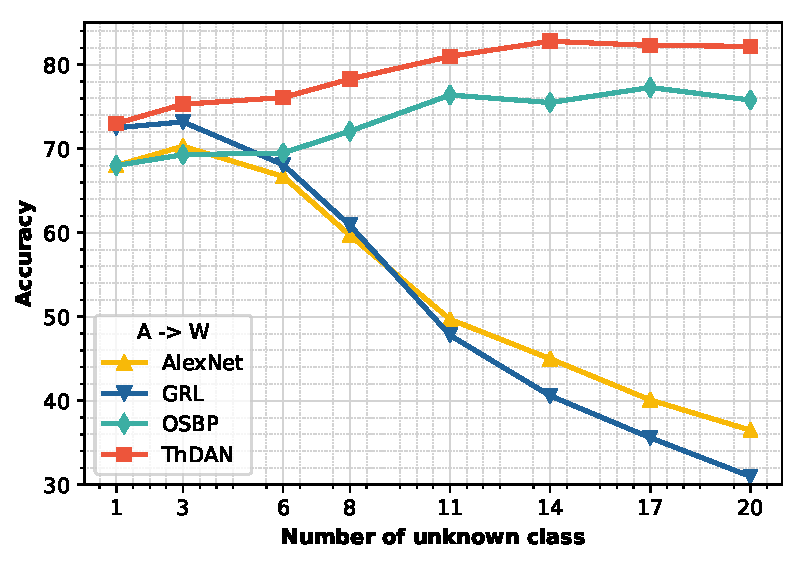
\includegraphics[width=0.33\textwidth]{contents/figures/pdf/analysis/class_change.pdf} 
        \label{figure: number of unknown class}
    }
    \subfloat[Accury \textit{w.r.t.} value of $\gamma_0$]{
        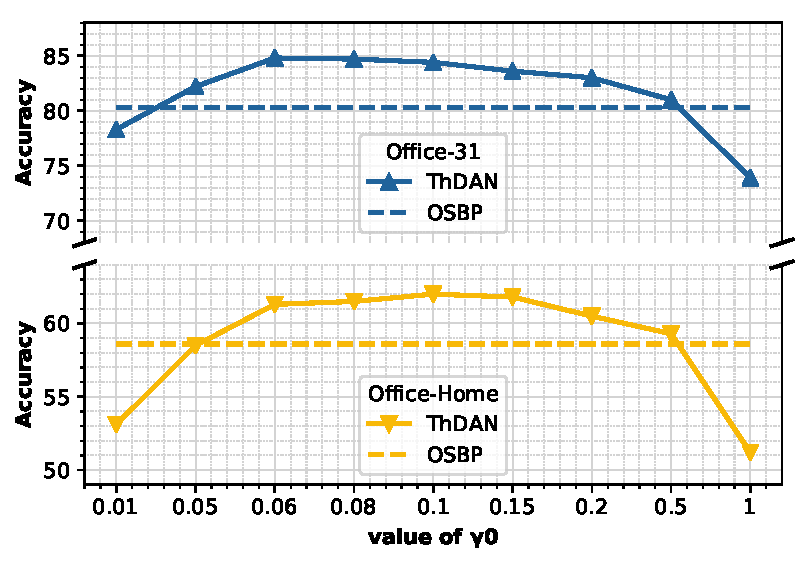
\includegraphics[width=0.33\textwidth]{contents/figures/pdf/analysis/sigma_change.pdf} 
        \label{figure: changing of sigma}
    }
    \\
    \caption{ }
    \label{figure: analysis}
\end{figure}

In the revised manuscript, the claim of \figurename{\ref{figure: analysis}} is modified for clearer representation.
The rewritten claim has been stated in the previous questions:
\begin{itemize}
    \item  In \textbf{Question \ref{Question: class number}}, we modify the claim of \figurename{\ref{figure: ration of unknown}} and \ref{figure: number of unknown class} by adding more analysis to explain how the performance changes with different sampling proportions between the data from known and unknown classes. 
    \item In \textbf{Question \ref{Question: threshold}}, we modify the claim of \figurename{\ref{figure: changing of sigma}} by providing a more detailed analysis on why the proposed method is insensitive to the setting of $\gamma_0$. 
\end{itemize}


% \begin{siderules}
%     \textit{
%         \footnotesize
%         (\textbf{a}):
%         The prediction accuracy of ThDAN when we changed the ratio of unknown samples in the adaptation task \textit{A$\to$D}.
%         (\textbf{b}):
%         The prediction accuracy of ThDAN when we changed the number of unknown classes in the adaptation task \textit{A$\to$W}.
%         (\textbf{c}): The prediction accuracy of ThDAN when we change the value of $\sigma_0$ on dataset Office-31 and Office-Home.
%     }
% \end{siderules}


\section{Some equations missed ``,'' or ``.'' at their ends.}
\subsection*{\underline{\textbf{Response:}}}

Thanks for your reminding.
The equations in the revised manuscript have been corrected.


